\begin{slide}{Back-Propagation in TensorFlow}
   \only<2>{
  \begin{figure}
  \centering
    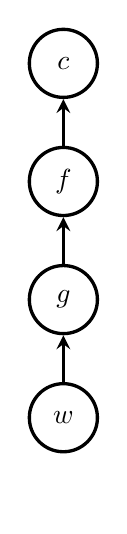
\begin{tikzpicture}
     % Nodes
      \path [very thick] (0, 0)
            coordinate [draw, circle, text width=0.6cm] (w) node {$w$};
      \path [very thick] (0, 1.5)
             coordinate [draw, circle, text width=0.6cm] (g) node {$g$};
      \path [very thick] (0, 3)
            coordinate [draw, circle, text width=0.6cm] (f) node {$f$};
      \path [very thick] (0, 4.5)
            coordinate [draw, circle, text width=0.6cm] (c) node {$c$};

      % Edges
      \draw [very thick, -stealth] (w) -- (g);
      \draw [very thick, -stealth] (g) -- (f);
      \draw [very thick, -stealth] (f) -- (c);

      % Placeholder
      \draw (0, -1.1);
  \end{tikzpicture}
  \end{figure}
  }
  \only<3>{
  \begin{figure}
  \centering
    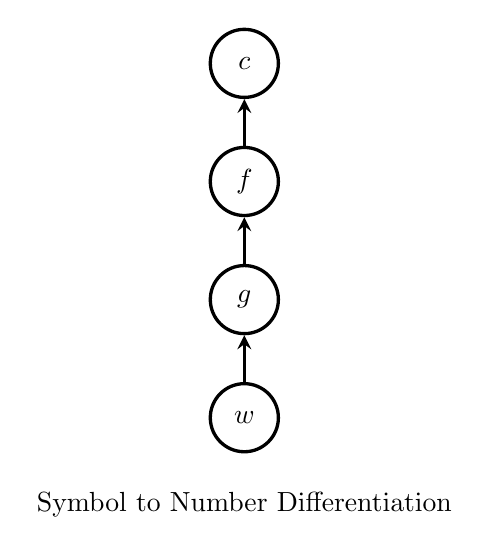
\begin{tikzpicture}
     % Nodes
      \path [very thick] (0, 0)
            coordinate [draw, circle, text width=0.6cm] (w) node {$w$};
      \path [very thick] (0, 1.5)
             coordinate [draw, circle, text width=0.6cm] (g) node {$g$};
      \path [very thick] (0, 3)
            coordinate [draw, circle, text width=0.6cm] (f) node {$f$};
      \path [very thick] (0, 4.5)
            coordinate [draw, circle, text width=0.6cm] (c) node {$c$};

      % Edges
      \draw [very thick, -stealth] (w) -- (g);
      \draw [very thick, -stealth] (g) -- (f);
      \draw [very thick, -stealth] (f) -- (c);

      % Label
     \draw (0, -1.1) node {Symbol to Number Differentiation};
  \end{tikzpicture}
  \end{figure}
  }
  \only<4>{
  \begin{figure}
  \centering
    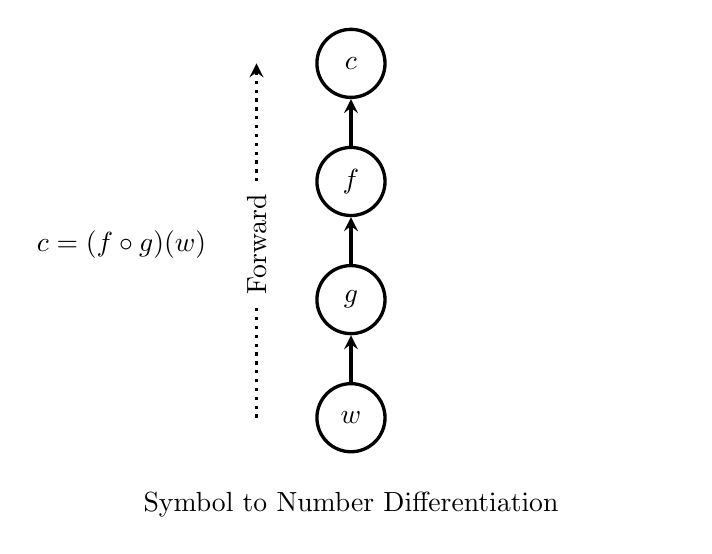
\begin{tikzpicture}
     % Nodes
      \path [very thick] (0, 0)
            coordinate [draw, circle, text width=0.6cm] (w) node {$w$};
      \path [very thick] (0, 1.5)
             coordinate [draw, circle, text width=0.6cm] (g) node {$g$};
      \path [very thick] (0, 3)
            coordinate [draw, circle, text width=0.6cm] (f) node {$f$};
      \path [very thick] (0, 4.5)
            coordinate [draw, circle, text width=0.6cm] (c) node {$c$};

      % Edges
      \draw [very thick, -stealth] (w) -- (g);
      \draw [very thick, -stealth] (g) -- (f);
      \draw [very thick, -stealth] (f) -- (c);

      % Forward Propagation
      \draw [very thick, -stealth, dotted]
            (-1.2, 0) -- +(0, 1.4)
            (-1.2, 3) -- +(0, 1.5);
      \draw (-1.2, 2.2) node [rotate=90] {Forward};
      \draw (-1.4, 2.2) node [left] {$c = (f \circ g)(w)\hspace{0.3cm}$};

      % Spacing
      \draw (4.2, 0);

      % Label
     \draw (0, -1.1) node {Symbol to Number Differentiation};
  \end{tikzpicture}
  \end{figure}
  }
  \only<5>{
  \begin{figure}
  \centering
    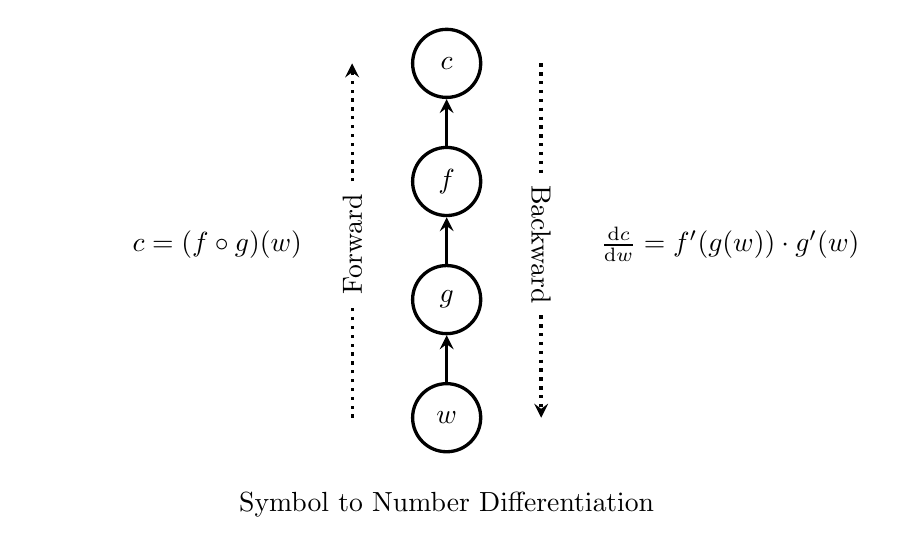
\begin{tikzpicture}
     % Nodes
      \path [very thick] (0, 0)
            coordinate [draw, circle, text width=0.6cm] (w) node {$w$};
      \path [very thick] (0, 1.5)
             coordinate [draw, circle, text width=0.6cm] (g) node {$g$};
      \path [very thick] (0, 3)
            coordinate [draw, circle, text width=0.6cm] (f) node {$f$};
      \path [very thick] (0, 4.5)
            coordinate [draw, circle, text width=0.6cm] (c) node {$c$};

      % Edges
      \draw [very thick, -stealth] (w) -- (g);
      \draw [very thick, -stealth] (g) -- (f);
      \draw [very thick, -stealth] (f) -- (c);

      % Forward Propagation
      \draw [very thick, -stealth, dotted]
            (-1.2, 0) -- +(0, 1.4)
            (-1.2, 3) -- +(0, 1.5);
      \draw (-1.2, 2.2) node [rotate=90] {Forward};
      \draw (-1.4, 2.2) node [left] {$c = (f \circ g)(w)\hspace{0.3cm}$};

      % Backward Propagation
      \draw [very thick, -stealth, dotted]
            (+1.2, 4.5) -- +(0, -1.4)
            (+1.2, 1.3) -- +(0, -1.3);
      \draw (+1.2, 2.2) node [rotate=270] {Backward};
      \draw (+3.6, 2.2) node {$\frac{\mathrm{d}c}{\mathrm{d}w} = f'(g(w)) \cdot g'(w)$};

     % Spacing
     \draw (-5.3, 0);

     % Label
     \draw (0, -1.1) node {Symbol to Number Differentiation};
  \end{tikzpicture}
  \end{figure}
  }
  \only<6>{
  \begin{figure}
  \centering
    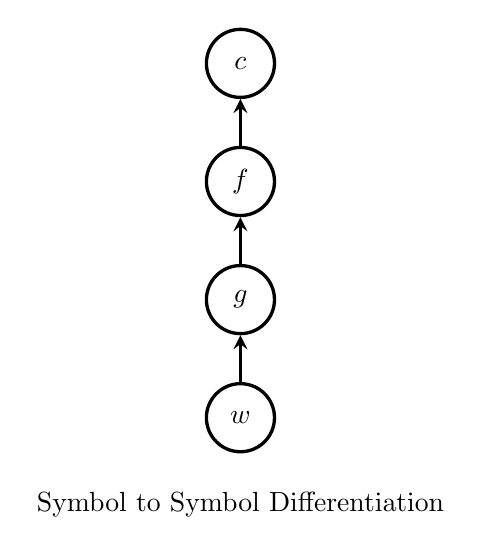
\begin{tikzpicture}
     % Nodes
      \path [very thick] (0, 0)
            coordinate [draw, circle, text width=0.6cm] (w) node {$w$};
      \path [very thick] (0, 1.5)
             coordinate [draw, circle, text width=0.6cm] (g) node {$g$};
      \path [very thick] (0, 3)
            coordinate [draw, circle, text width=0.6cm] (f) node {$f$};
      \path [very thick] (0, 4.5)
            coordinate [draw, circle, text width=0.6cm] (c) node {$c$};

      % Edges
      \draw [very thick, -stealth] (w) -- (g);
      \draw [very thick, -stealth] (g) -- (f);
      \draw [very thick, -stealth] (f) -- (c);

      % Label
     \draw (0, -1.1) node {Symbol to Symbol Differentiation};
  \end{tikzpicture}
  \end{figure}
  }
  \only<7>{
  \begin{figure}
  \centering
    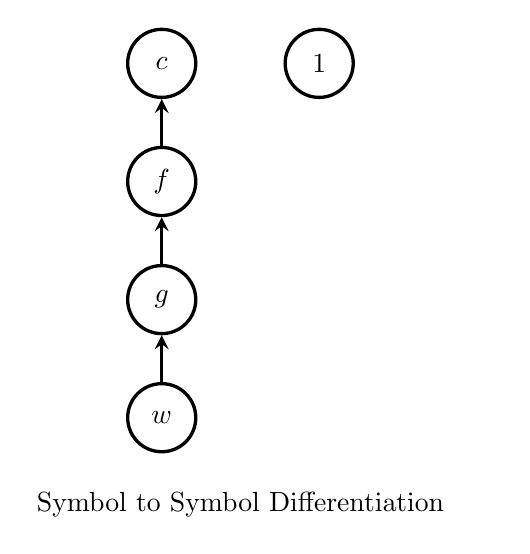
\begin{tikzpicture}
     % Nodes
      \path [very thick] (0, 0)
            coordinate [draw, circle, text width=0.6cm] (w) node {$w$};
      \path [very thick] (0, 1.5)
             coordinate [draw, circle, text width=0.6cm] (g) node {$g$};
      \path [very thick] (0, 3)
            coordinate [draw, circle, text width=0.6cm] (f) node {$f$};
      \path [very thick] (0, 4.5)
            coordinate [draw, circle, text width=0.6cm] (c) node {$c$};

      % Edges
      \draw [very thick, -stealth] (w) -- (g);
      \draw [very thick, -stealth] (g) -- (f);
      \draw [very thick, -stealth] (f) -- (c);

      % Gradient Nodes
      \path [very thick] (2, 4.5)
            coordinate [draw, circle, text width=0.6cm] (dc) node {$1$};

     % Label
     \draw (1, -1.1) node {Symbol to Symbol Differentiation};

     % Spacing
     \draw (4.3, 0);
  \end{tikzpicture}
  \end{figure}
  }
  \only<8>{
  \begin{figure}
  \centering
    \tikzset{every picture/.style=very thick}
    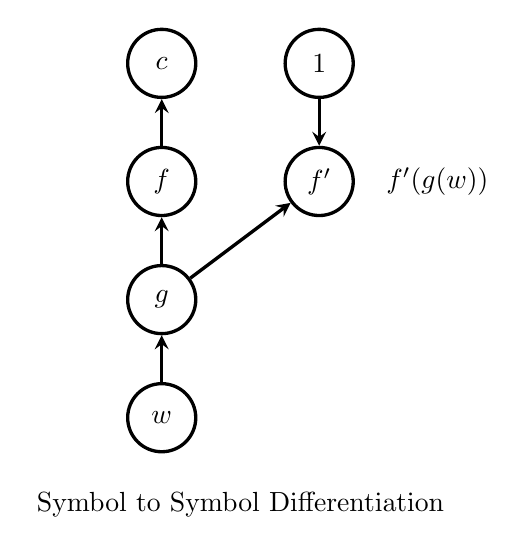
\begin{tikzpicture}
     % Nodes
      \path (0, 0) coordinate [draw, circle, text width=0.6cm] (w) node {$w$};
      \path (0, 1.5) coordinate [draw, circle, text width=0.6cm] (g) node {$g$};
      \path (0, 3) coordinate [draw, circle, text width=0.6cm] (f) node {$f$};
      \path (0, 4.5) coordinate [draw, circle, text width=0.6cm] (c) node {$c$};

      % Edges
      \draw [-stealth] (w) -- (g);
      \draw [-stealth] (g) -- (f);
      \draw [-stealth] (f) -- (c);

      % Gradient Nodes
      \path (2, 4.5) coordinate [draw, circle, text width=0.6cm] (dc) node {$1$};
      \path (2, 3) coordinate [draw, circle, text width=0.6cm] (df) node {$f'$};

      % Gradient Edges
      \draw [-stealth] (dc) -- (df);
      \draw [-stealth] (g) -- (df);

      % Gradient Labels
      \draw (3.5, 3) node {$f'(g(w))$};

     % Label
     \draw (1, -1.1) node {Symbol to Symbol Differentiation};

     % Spacing
     \draw (-1.5, 0);
  \end{tikzpicture}
  \end{figure}
  }
  \only<9>{
  \begin{figure}
  \centering
    \tikzset{every picture/.style=very thick}
    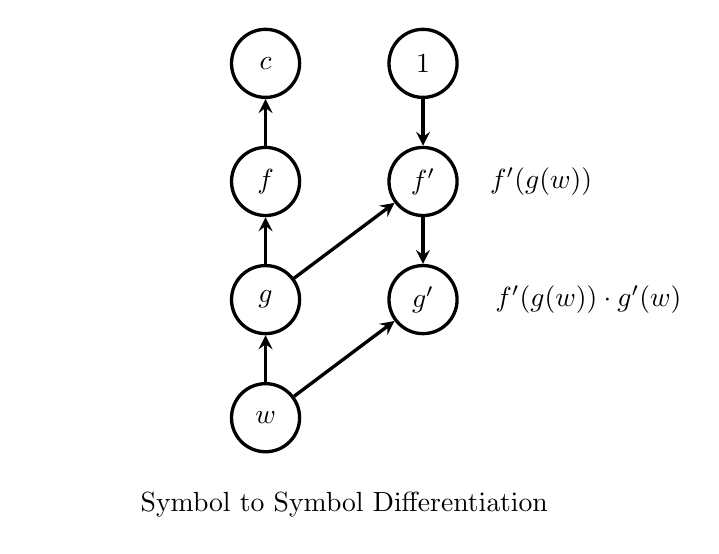
\begin{tikzpicture}
     % Nodes
      \path (0, 0) coordinate [draw, circle, text width=0.6cm] (w) node {$w$};
      \path (0, 1.5) coordinate [draw, circle, text width=0.6cm] (g) node {$g$};
      \path (0, 3) coordinate [draw, circle, text width=0.6cm] (f) node {$f$};
      \path (0, 4.5) coordinate [draw, circle, text width=0.6cm] (c) node {$c$};

      % Edges
      \draw [-stealth] (w) -- (g);
      \draw [-stealth] (g) -- (f);
      \draw [-stealth] (f) -- (c);

      % Gradient Nodes
      \path (2, 4.5) coordinate [draw, circle, text width=0.6cm] (dc) node {$1$};
      \path (2, 3) coordinate [draw, circle, text width=0.6cm] (df) node {$f'$};
      \path (2, 1.5) coordinate [draw, circle, text width=0.6cm] (dg) node {$g'$};

      % Gradient Edges
      \draw [-stealth] (dc) -- (df);
      \draw [-stealth] (g) -- (df);
      \draw [-stealth] (df) -- (dg);
      \draw [-stealth] (w) -- (dg);

      % Gradient Labels
      \draw (3.5, 3) node {$f'(g(w))$};
      \draw (4.1, 1.5) node {$f'(g(w)) \cdot g'(w)$};

     % Label
     \draw (1, -1.1) node {Symbol to Symbol Differentiation};

     % Spacing
     \draw (-3, 0);
  \end{tikzpicture}
  \end{figure}
  }
  \only<10>{
  \begin{figure}
  \centering
    \tikzset{every picture/.style=very thick}
    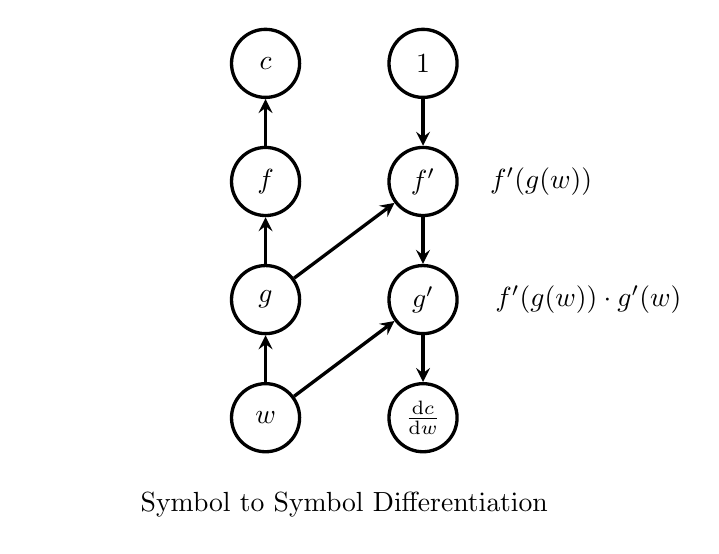
\begin{tikzpicture}
     % Nodes
      \path (0, 0) coordinate [draw, circle, text width=0.6cm] (w) node {$w$};
      \path (0, 1.5) coordinate [draw, circle, text width=0.6cm] (g) node {$g$};
      \path (0, 3) coordinate [draw, circle, text width=0.6cm] (f) node {$f$};
      \path (0, 4.5) coordinate [draw, circle, text width=0.6cm] (c) node {$c$};

      % Edges
      \draw [-stealth] (w) -- (g);
      \draw [-stealth] (g) -- (f);
      \draw [-stealth] (f) -- (c);

      % Gradient Nodes
      \path (2, 4.5) coordinate [draw, circle, text width=0.6cm]
            (dc) node {$1$};
      \path (2, 3) coordinate [draw, circle, text width=0.6cm]
            (df) node {$f'$};
      \path (2, 1.5) coordinate [draw, circle, text width=0.6cm]
            (dg) node {$g'$};
      \path (2, 0) coordinate [draw, circle, text width=0.6cm]
           (dw) node {$\frac{\mathrm{d}c}{\mathrm{d}w}$};

      % Gradient Labels
      \draw (3.5, 3) node {$f'(g(w))$};
      \draw (4.1, 1.5) node {$f'(g(w)) \cdot g'(w)$};

      % Gradient Edges
      \draw [-stealth] (dc) -- (df);
      \draw [-stealth] (g) -- (df);
      \draw [-stealth] (df) -- (dg);
      \draw [-stealth] (w) -- (dg);
      \draw [-stealth] (dg) -- (dw);

     % Label
     \draw (1, -1.1) node {Symbol to Symbol Differentiation};

     % Spacing
     \draw (-3, 0);
  \end{tikzpicture}
  \end{figure}
  }
\end{slide}

%%% Local Variables:
%%% mode: latex
%%% TeX-master: "../presentation.tex"
%%% End:
